\chapter{آزمایش‌ها، نتیجه‌گیری و پیشنهادها}
%%%%%%%%%%%%%%%%%%%%%%%%%%%%%%%%%%%%%%%%%%%
با بررسی گسترده‌ای که روی مدل‌های کیفیتی انجام گرفت، این نتیجه واضح و مبرهن شد که استفاده‌پذیری یکی از اصول کیفیتی انکارناپذیر نرم‌افزار است؛ اما هنوز در روزگار فعلی و با گذشت حدود چهل سال از معرفی اولین مدل کیفیتی نرم‌افزار، همچنان شاهد وجود و حتی تولید ابزارهایی غیرقابل استفاده و در نتیجه بی‌کیفیت در صنعت نرم‌افزار هستیم. مطالعه‌ای دیگر روی سامانه‌های مبتنی بر وب نشان می‌دهد که امروزه بسیاری از امور مربوط به اداره‌ها، زندگی روزمره و امور جوامع، وابسته به این سامانه‌ها شده و بسیاری از کسب‌وکارها حول خدمات تحت وب به وجود آمده‌اند؛ بنابراین بدیهی به نظر می‌رسد که استفاده‌ناپذیری و کیفیت پایین به منزله ضرر بیشتر و از دست دادن کاربران و مصرف‌کنندگان برای صنایع، و همچنین دشوارتر شدن دسترسی به خدمات با کیفیت، برای جامعه مصرف‌کنندگان خواهد بود. به منظور افزایش استفاده‌پذیری سامانه‌های مبتنی بر وب، می‌بایست با مطالعه مدل‌های کیفیتی و همچنین پژوهش‌هایی که حول ناکارآمدی بسیاری از این مدل‌ها انجام شده‌اند، به دلیل راه‌حل باشیم. مدلی که در سال ۲۰۱۳ و توسط آقایان تولیس و آلبرت در کتاب «اندازه‌گیری تجربه کاربری: جمع‌آوری، تحلیل و ارائه خصیصه‌های استفاده‌پذیری»
\cite{albert_measuring_2013}
اثبات شد که جنبه‌های وسیع‌تری از استفاده‌پذیری را، در عین کارآمد بودن برای بسیاری از سازمان‌ها، مورد پوشش خود قرار می‌دهد. بنابراین ده سناریو توسط ایشان مطرح شدند که بیشترین تمرکز را در مطالعات استفاده‌پذیری داشتند که در این پروژه نیز تمرکز روی این ده سناریو بود.\\
در طول فصل سوم می‌توان به این نتیجه رسید که ده سناریوی مطرح شده به منظور مطالعه استفاده‌پذیری، پوشا بوده و طبق مدل کیفیتی انتخاب شده، جنبه‌ای نخواهد ماند که طبق این سناریوها پوشش داده نشود؛ از طرفی نیز به منظور مطالعه این سناریوهای مطرح، با بررسی ۸۳ ابزار مطرح در حوزه مطالعه و سنجش استفاده‌پذیری، مشاهده می‌شود که الگوهای مشابهی برای این کار وجود دارد که البته هر ابزار در عین داشتن جزئیاتی خرد، دارای ماموریت و هدفی مشابه با بقیه‌، در مطالعه هر یک از این سناریوها هستند؛ بنابراین به مطالعه الگوهای استفاده شده در ابزارهای مطرح پرداختیم و هشت الگوی شاخص\RTLfootnote{با تقریب خوبی، در تمام ابزارها ردی از این هشت الگو یافت می‌شد؛ بسیاری از ابزارهایی که یکی دو الگو را نمی‌توانستند پوشش دهند، در لیست تغییرات خود و همچنین در برنامه بلند مدت خود، در نظر داشتند که به افق تعیین شده و پوشش حداکثری الگوها به منظور انجام تمامی سناریوها دست پیدا کنند.}
یافته شد. این الگوها که در فصل سوم به تفصیل شرح داده شده‌اند، سنگ بنای بسیاری از ابزارهای فعلی هستند که ما به عنوان ابزارهای مطالعه استفاده‌پذیری میشناسیم. با در نظر گرفتن این ۸۳ ابزار و همچنین الگوهای یاد شده، به ساختن موارد تست پرداختیم و در ابتدا سعی کردیم موارد تست خود را بیشتر مورد ایده‌پردازی قرار دهیم؛ سپس نیازمندی‌ها را مهندسی کرده و پس از شناخت دقیق آن‌ها، وارد فاز پیاده‌سازی شدیم و ابزار هدف ساخته شد.
\section{آزمایش‌ها}
با پیاده‌سازی ابزار، شروع به انجام چندین مورد آزمایش کردیم که در ادامه توضیحات مربوط به هرکدام و شکل‌های مربوط به هرکدام درج شده است.
\begin{figure}
	\centering
	\subfloat[شروع انجام آزمون]{
		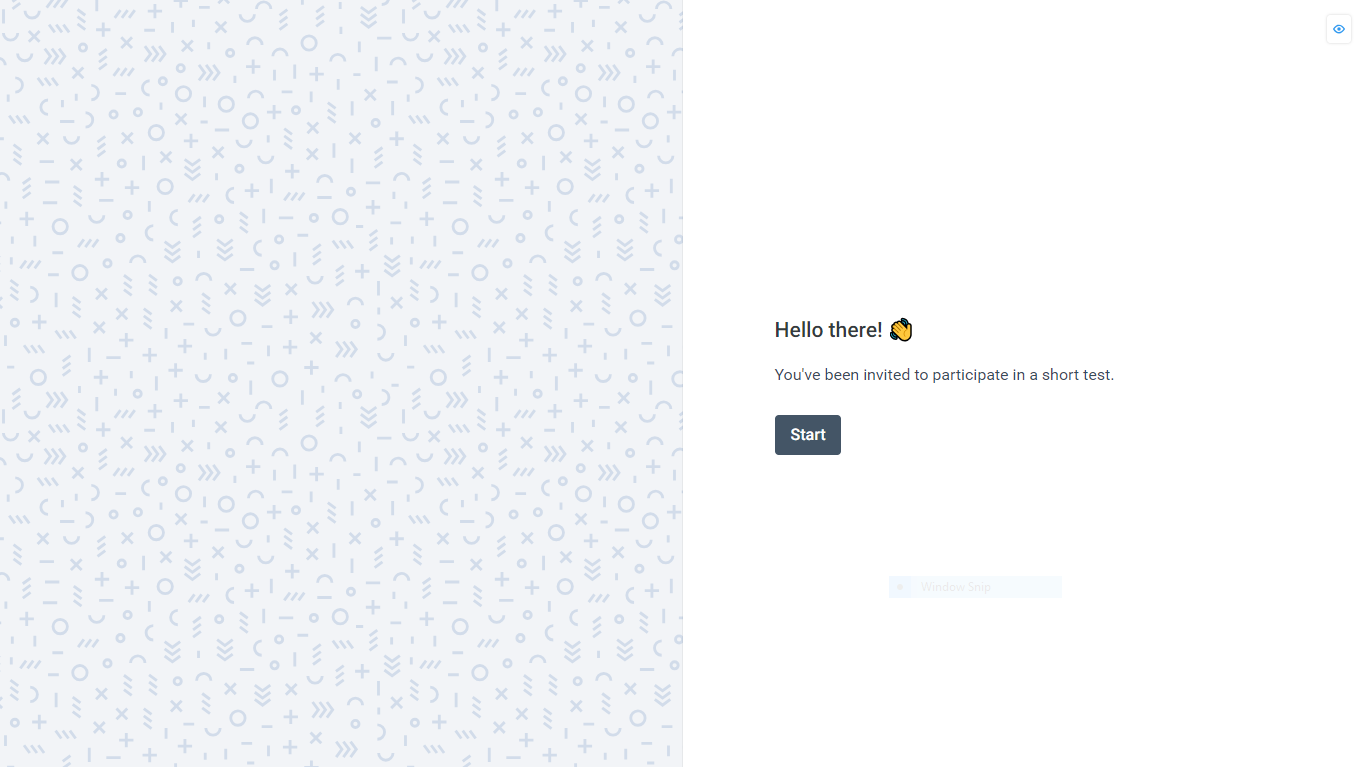
\includegraphics[width=5cm]{Resources/test1-1.PNG}
	}
	\hspace{0mm}
	\subfloat[انجام آزمون ۵ ثانیه روی یک طراحی آزمایشی، برای بررسی تاثیر طراحی در یادگیری‌پذیری]{
		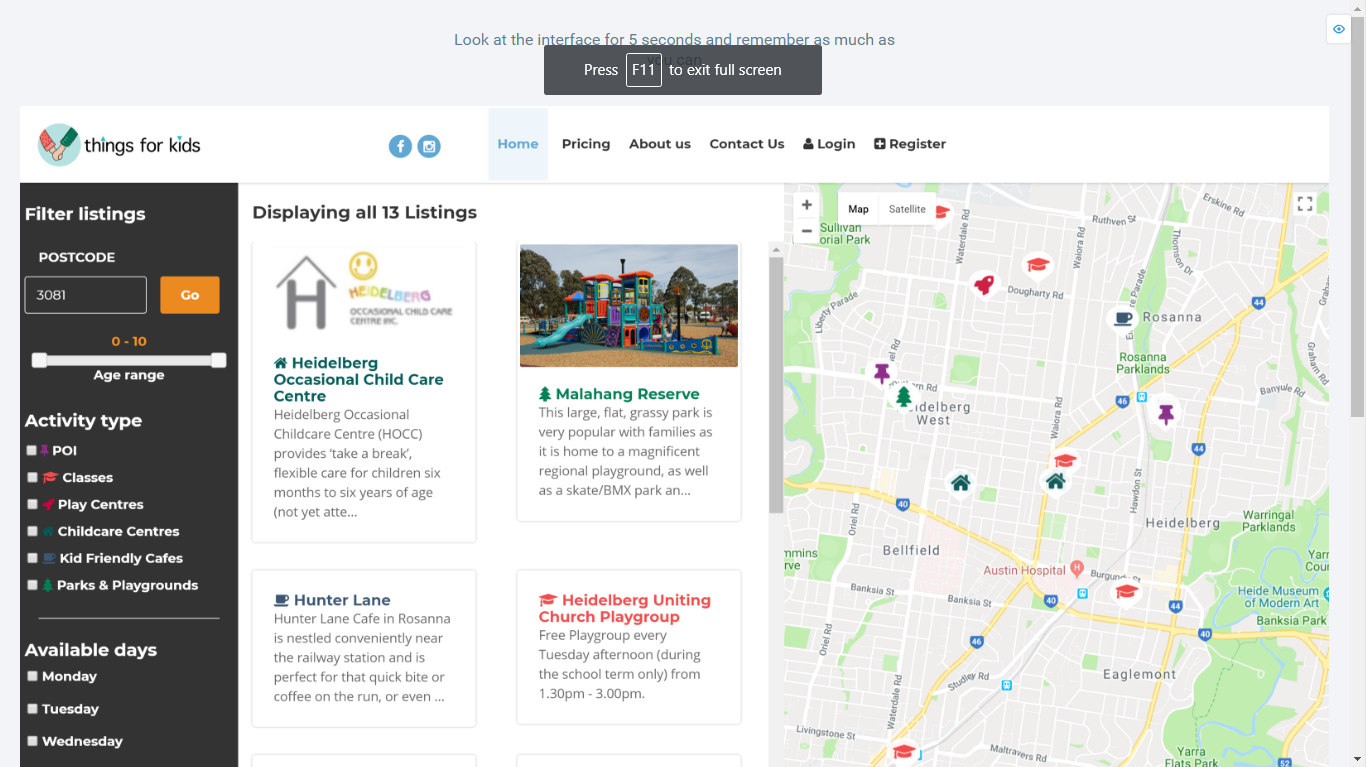
\includegraphics[width=9cm]{Resources/test1-2.PNG}
	}
	\hspace{0mm}
	\subfloat[پرسیدن سوال اول مربوط به طراحی]{
		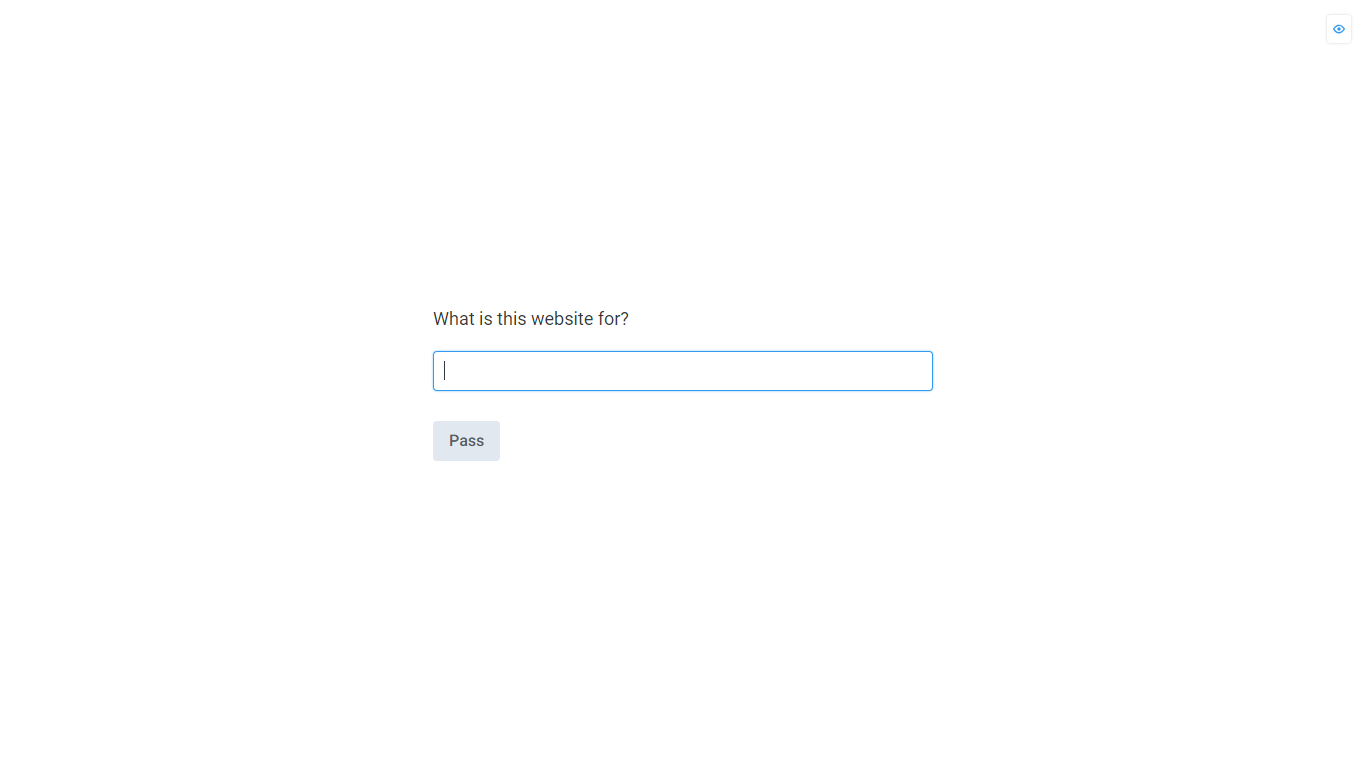
\includegraphics[width=7cm]{Resources/test1-3.PNG}
	}
	\subfloat[پرسیدن سوال دوم مربوط به طراحی]{
		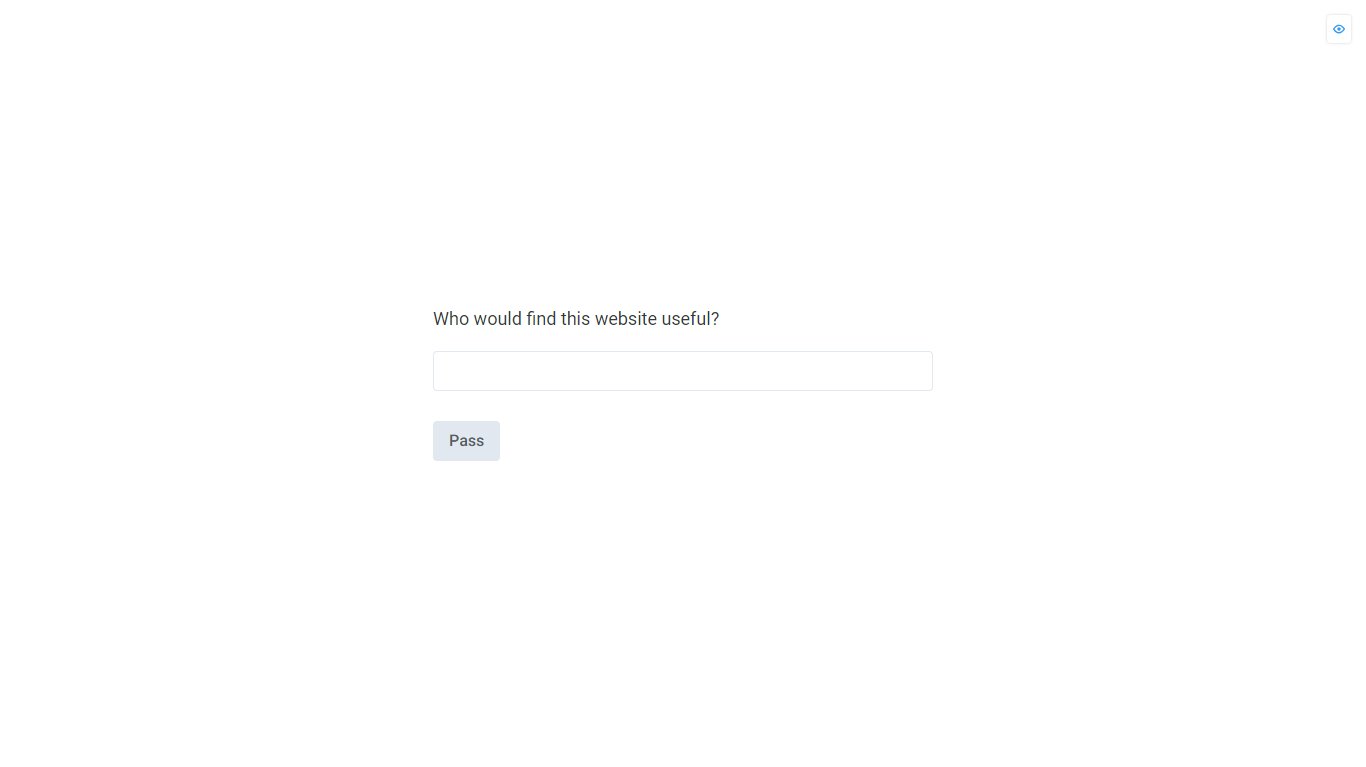
\includegraphics[width=7cm]{Resources/test1-4.PNG}
	}
	\caption{انجام آزمایشی برای بررسی یادگیری‌پذیری}
	\label{fig:5sec}
\end{figure}
همانطور که در شکل
\ref{fig:5sec}
مشاهده می‌شود، آزمونی روی یک طرح مفهومی انجام شده است تا یادگیری‌پذیری و همچنین شلوغ‌بودن طراحی مورد سنجش واقع شود. طی این آزمون شرکت‌کننده در آزمون به مدت ۵ ثانیه در معرض تصویر یاد شده در شکل قرار می‌گیرد و پس از آن، طبق دستورالعمل مطرح شده، سوالاتی از وی پرسیده می‌شود که می‌تواند چندین حالت مختلف برای پاسخ‌دهی داشته باشد؛ در این مورد، نوع پاسخ‌دهی، پاسخ کوتاه انتخاب شده.
\begin{figure}
	\centering
	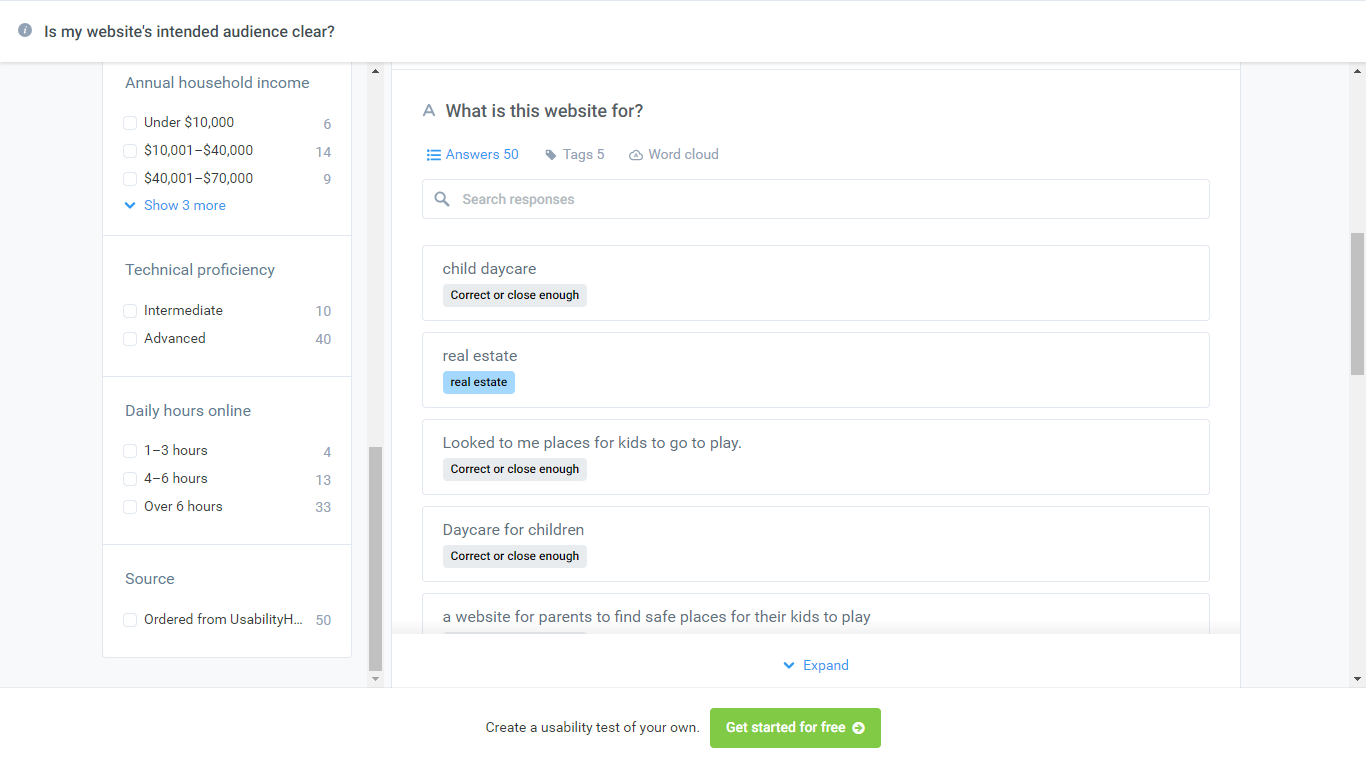
\includegraphics[width=11cm]{Resources/res1.PNG}
	\caption{نتایج مربوط به آزمون مطرح شده در شکل \ref{fig:5sec}}
	\label{fig:res}
\end{figure}
نتایج تجمیع‌شده و یکپارچه آزمون مطرح شده در شکل
\ref{fig:5sec}،
در شکل
\ref{fig:res}
قابل مشاهده‌اند.
\begin{figure}
	\centering
	\subfloat[شروع انجام آزمون]{
		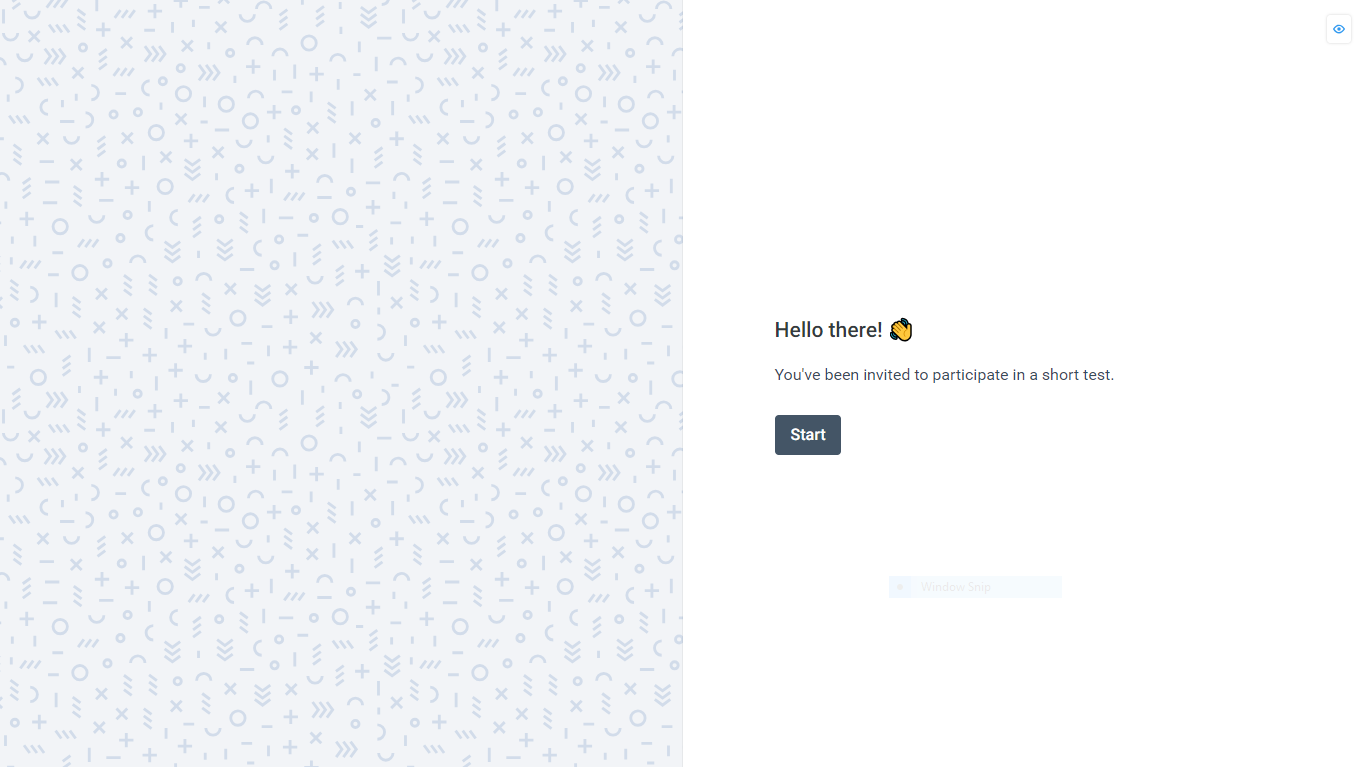
\includegraphics[width=5cm]{Resources/test1-1.PNG}
	}
	\hspace{0mm}
	\subfloat[آزمونی برای بررسی نحوه پیمایش کاربران در صفحه نمایش]{
		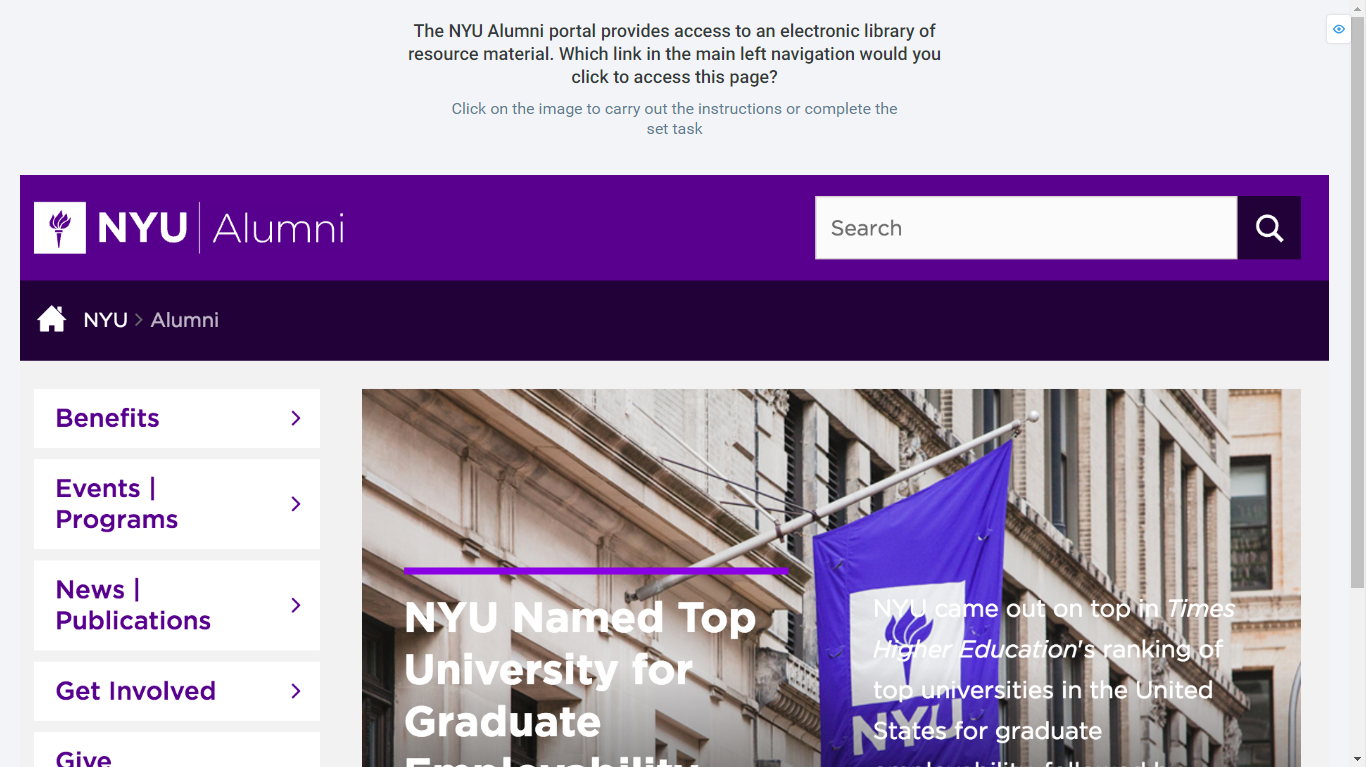
\includegraphics[width=9cm]{Resources/test3-1.PNG}
	}
	\hspace{0mm}
	\subfloat[پرسیدن سوال مربوط به پیمایش]{
		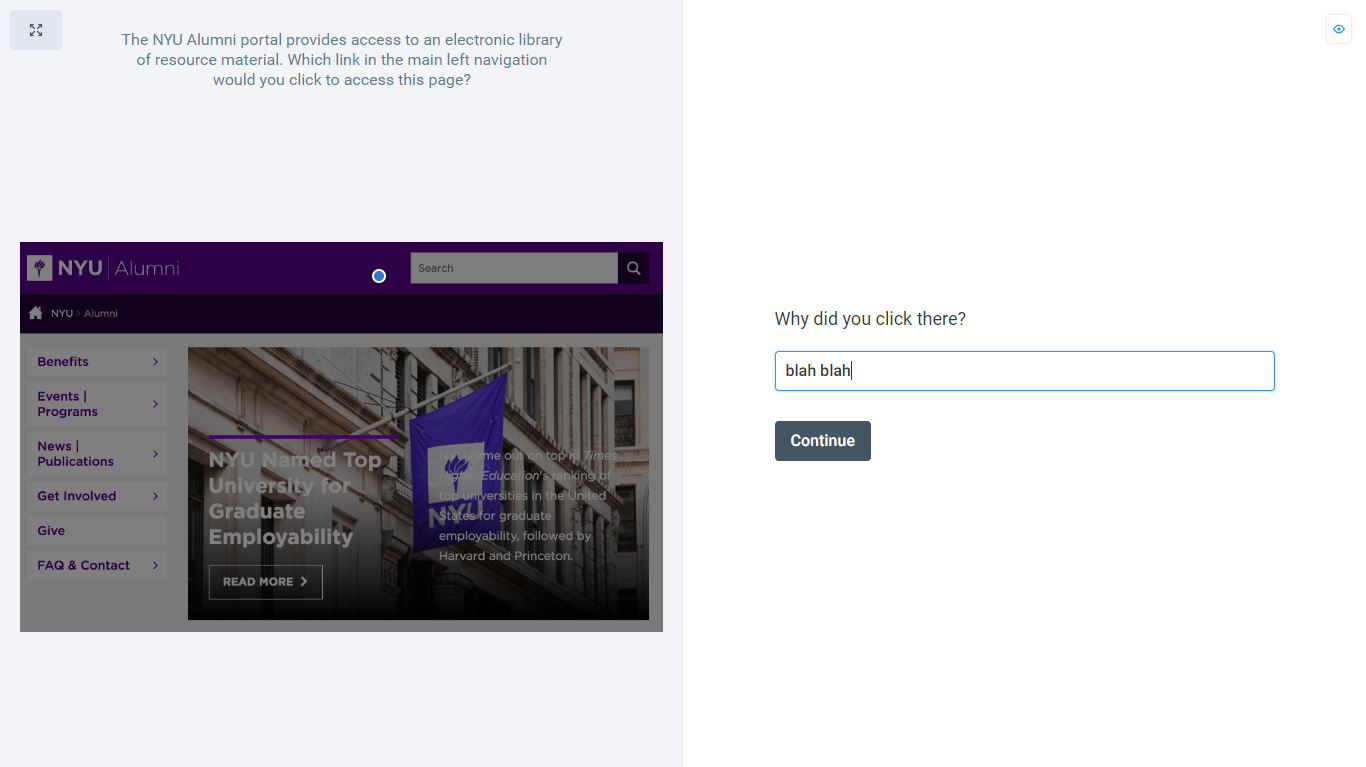
\includegraphics[width=6cm]{Resources/test3-2.PNG}
	}
	\hspace{0mm}
	\subfloat[پرسش از سوال مربوط به ترجیح کاربران]{
		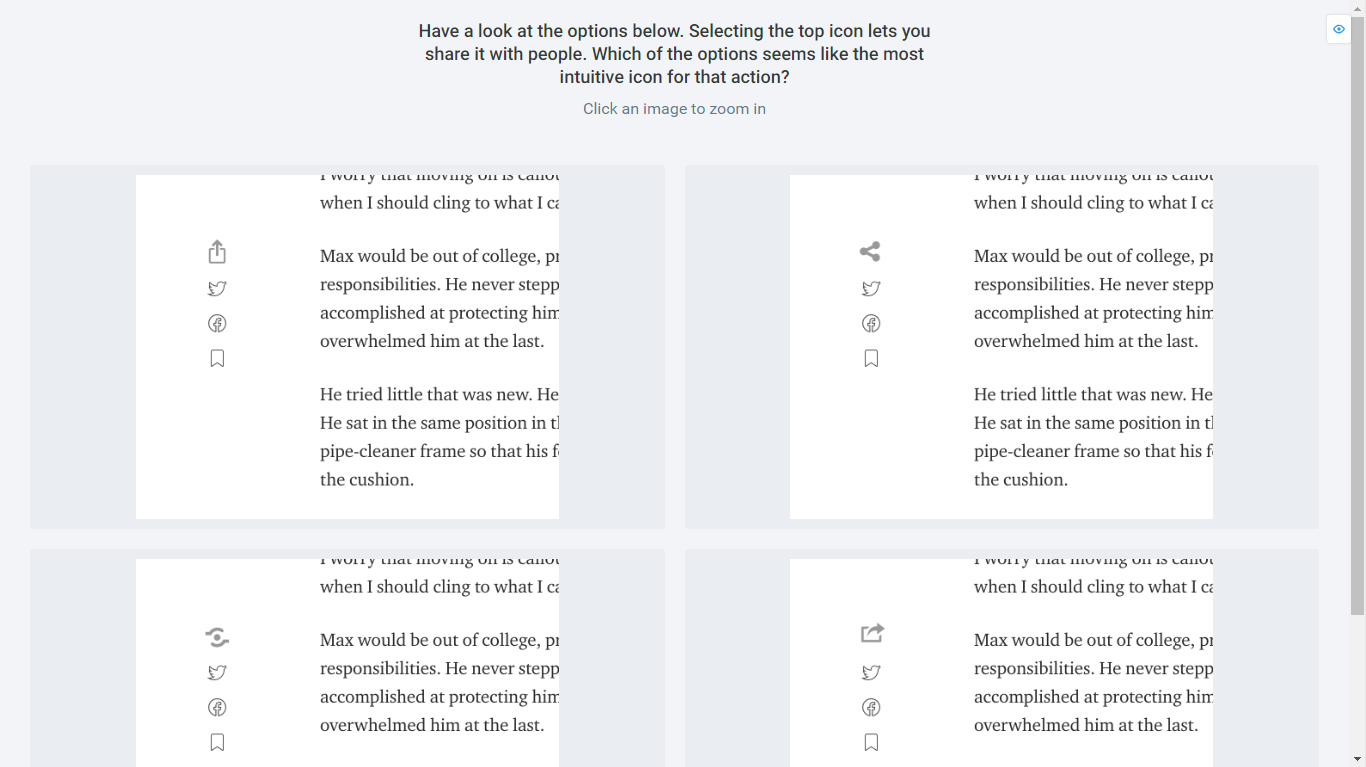
\includegraphics[width=6cm]{Resources/test2-1.PNG}
	}
	\caption{انجام آزمونی برای سنجش نحوه پیمایش و ترجیح کاربران}
	\label{fig:test2}
\end{figure}
همچنین مطابق شکل
\ref{fig:test2}
آزمون‌های بررسی نحوه پیمایش و نیز ترجیح کاربران در رابطه با وبسایت فارغ‌التحصیلان دانشگاه نیویورک طرح و بررسی شد.
\section{نتیجه‌گیری}
حجم مطالعات انجام شده نشان دهنده پوشش جامعی از ابزارهای مطرح در حوزه سنجش استفاده‌پذیری است که علی‌رغم جستجوی بسیار برای داده‌ محک، نتیجه‌ای نیافتیم؛ در نهایت برای بیان اثبات برتری ابزار پیاده‌سازی شده با سایر ابزارها، به مطالعات خود بسنده می‌کنیم که در فصل سوم مورد بحث قرار گرفتند. طبق این مطالعات، تعداد بسیار کمی از ابزارهای موجود می‌توانند تمامی سناریو‌های مطرح برای استفاده‌پذیری را مورد پوشش قرار دهند که می‌توان با مراجعه به جدول
\ref{tab:tools}
به این نتیجه رسید. ابزار پیاده‌سازی شده طی این پروژه، علاوه بر اینکه می‌تواند تمامی سناریوهای قابل انجام برای مطالعه استفاده‌پذیری را پوشش دهد، امکان مشخص ساختن آستانه کیفیت\LTRfootnote{Quality Threshold}
کارگران جمع‌سپاری را نیز فراهم می‌آورد که این مورد در سایر ابزارهای مشابه نبود؛ درواقع ابزار حاضر، تنها ابزاری است که به آزمون‌گر اجازه استفاده از دو روش جمع‌سپاری (جمع‌سپاری با استفاده از رابط خود ابزار و سکوی داخلی ابزار) و همچنین جمع‌سپاری با استفاده از یک سکوی خارج از سامانه (سکوی
«\lr{Figure-Eight}»)
را به آزمون‌گر می‌دهد. البته شایان ذکر است که از سکوهای جمع‌سپاری‌ای همچون
«\lr{Amazon Mechanical Turk}»،
به صورت موردی\LTRfootnote{Ad-hoc}
نیز برای انجام مطالعات استفاده‌پذیری، بهره برده‌اند. منتها باید توجه کرد که طبق مطالعات انجام شده در این پروژه، ابزاری که به طور خاص برای مطالعه استفاده‌پذیری توسعه داده شده و دارای قابلیت تغییر آستانه کیفیت مورد نیاز باشد، وجود نداشته است.
\section{پیشنهادها و کارهای آینده}
همانطور که در انتهای فصل سوم گفته شد، استفاده از روش مدل‌سازی کارگران برای کنترل کیفیت داده‌های حاصل از جمع‌سپاری، ساده‌ترین و کم‌هزینه‌ترین روش بود که طی آن، سنجش‌گر صرفا آستانه کیفیتی را مشخص می‌کند که پاسخ‌های دارای کیفیت کم‌تر از آن، از گردونه محاسبات خارج شده و بی‌تاثیر خواهند شد. اما می‌توان روش‌های پیچیده‌تر را نیز استفاده کرد که شاید برخی نیازمند پروفایل‌سازی از کاربران و یا مستلزم سایر نیازمندی‌های پیچیده‌تر باشد. همچنین با توجه به ظاهر ابتدایی ابزار و نمونه اولیه بودن آن، یکی از پتانسیل‌های توسعه این ابزار نیز می‌تواند توسعه در ابعاد ظاهری و زیبایی باشد.\\
علاوه بر موارد پیشین، می‌توان طی پروژه‌ای، با جزییات بیشتری ۸۳ ابزار مطرح شده در این پروژه را مورد بررسی قرار داده و مجموعه داده محکی برای آن‌ها فراهم آورد تا بتوان ابزارهای جدید را نیز به شیوه مستندتری بررسی کرد. همچنین گفتنی است که همانطوری که در فصل‌های اول گفته شد، این پروژه و محصول نهایی آن (ابزار تولید شده) می‌تواند پتانسیل تجاری خوبی برای سازمان‌ها و شرکت‌های بزرگ باشد تا ایده‌ای همانند ری‌کپچای گوگل را برای کاربردهای دیگر، از جمله سنجش رابط کاربری در ابعاد کوچک‌تر و آزمایش‌های خردتر، پیاده کرد.